% Template for PLoS
% Version 1.0 January 2009
%
% To compile to pdf, run:
% latex plos.template
% bibtex plos.template
% latex plos.template
% latex plos.template
% dvipdf plos.template

\documentclass[10pt]{article}

% amsmath package, useful for mathematical formulas
\usepackage{amsmath}
% amssymb package, useful for mathematical symbols
\usepackage{amssymb}

% graphicx package, useful for including eps and pdf graphics
% include graphics with the command \includegraphics
\usepackage{graphicx}

% cite package, to clean up citations in the main text. Do not remove.
\usepackage{cite}

\usepackage{color} 

% Use doublespacing - comment out for single spacing
\usepackage{setspace} 
\doublespacing


% Text layout
\topmargin 0.0cm
\oddsidemargin 0.5cm
\evensidemargin 0.5cm
\textwidth 16cm 
\textheight 21cm

% Bold the 'Figure #' in the caption and separate it with a period
% Captions will be left justified
\usepackage[labelfont=bf,labelsep=period,justification=raggedright]{caption}

% Use the PLoS provided bibtex style
\bibliographystyle{plos2009}

% Remove brackets from numbering in List of References
\makeatletter
\renewcommand{\@biblabel}[1]{\quad#1.}
\makeatother


% Leave date blank
\date{}

\pagestyle{myheadings}
%% ** EDIT HERE **


%% ** EDIT HERE **
%% PLEASE INCLUDE ALL MACROS BELOW

%% END MACROS SECTION

\begin{document}


%\section*{Tables}
%\begin{table}[!ht]
%\caption{
%\bf{Table title}}
%\begin{tabular}{|c|c|c|}
%table information
%\end{tabular}
%\begin{flushleft}Table caption
%\end{flushleft}
%\label{tab:label}
% \end{table}

\begin{table}[ht]
\caption{
\bf{Comparison of Hand-Written and Generated Code Counts.}}
\begin{tabular}{l c c c c c c}

    {\bf Language:}
    & {\bf C (H)}
    & {\bf C (G)}
    & {\bf Perl (H)}
    & {\bf Perl (G)}
    & {\bf Python (H)}
    & {\bf Python (G)} \\

    {\bf Model\,Container}
    & 1,832,580
    & 4,416,163
    & 30,406
    & 207,638
    & 14,568
    & 250,178 \\

    {\bf Heccer}
    & 1,163,991
    & 1,575,615
    & 57,565
    & 107,261
    & 1,586
    & 171,219 \\

    {\bf NS-SLI}
    & 1,448,636
    & 483,641
    & 4,603
    & 2,802
    & ---
    & --- \\

    {\bf SSP}
    & 829
    & 2,323
    & 55,063
    & ---
    & ---
    & --- \\

    {\bf Studio}
    & ---
    & ---
    & 174,923
    & ---
    & ---
    & --- \\

    {\bf G-Shell}
    & ---
    & ---
    & 28,142
    & ---
    & 623
    & 836 \\
\end{tabular}
\begin{flushleft} A comparison of hand-written (H) and automatically generated (G) code that supports the functionality of the independent components of the GENESIS simulation platform. Software hand-written in a system programming language such as C contains many more lines of code than the equivalent functionality replicated in a scripting language. The number of automatically generated lines of code is considerably greater than those written by hand.
\end{flushleft}
\label{tab:cbi-codecounts}
\end{table}

\clearpage

%\begin{figure}[ht]
%\begin{center}
%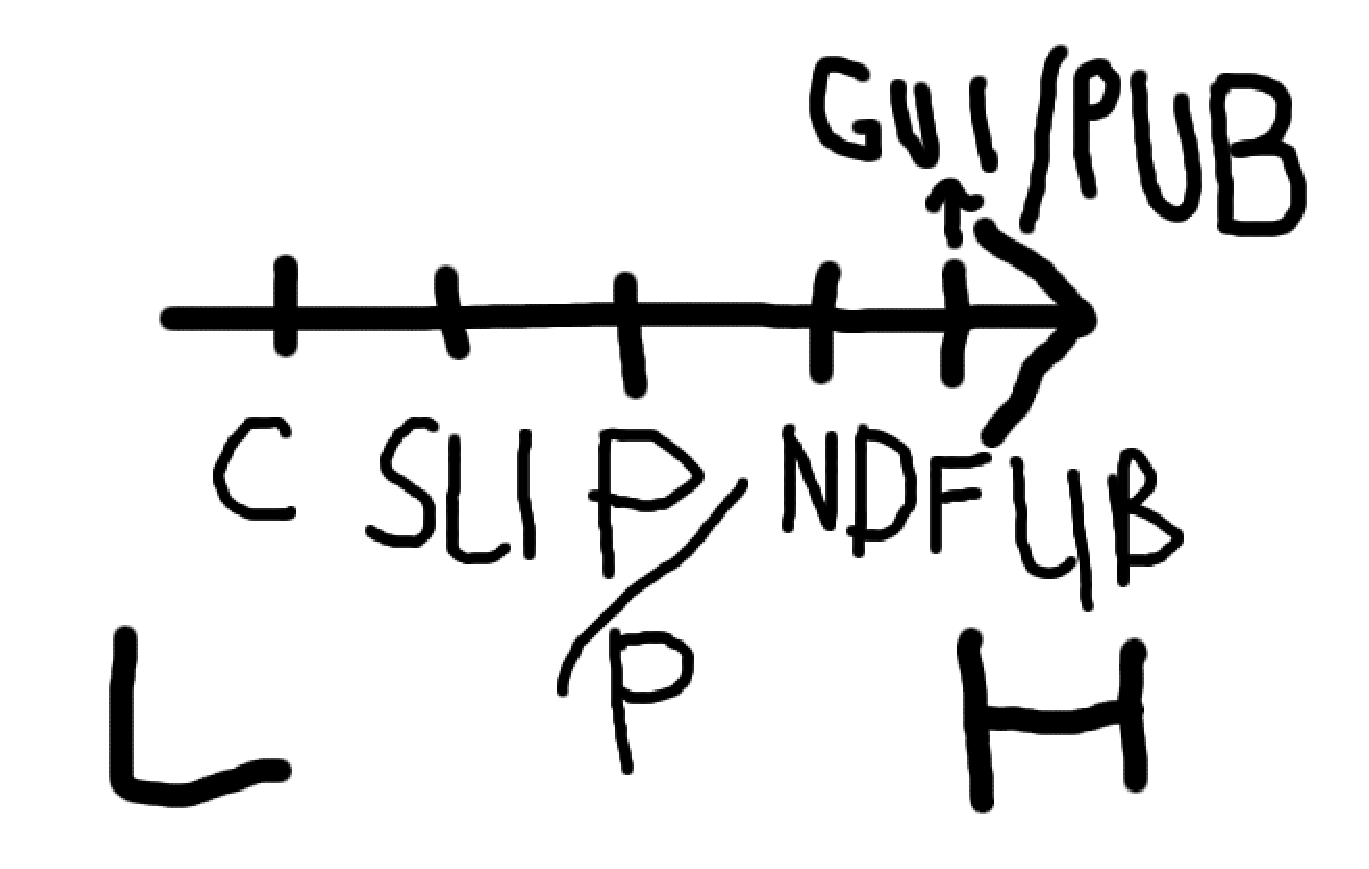
\includegraphics[width=4in]{figures/conceptual-hierarchy.eps}
%\end{center}
%\caption{
%{\bf Relationship Hierarchy between GENESIS Configurability and Extenxibility Options.}
%}
%\label{fig:conceptual-hierachy}
%\end{figure}


\end{document}
